\section{Motoren} \label{sec:motors}

\subsection{Schrittmotor}
Der Schrittmotor dient der Ausrichtung der Abschussvorrichtung bzw. der
Plattform, welche die Abschussvorrichtung trägt. Dieser Motor muss
daher die folgenden zwei Kriterien erfüllen.

\begin{itemize}
	\item Genauigkeit -- Der Motor richtet die Schussvorrichtung auf
		das Zielobjekt und hat somit direkten Einfluss auf die
		Genauigkeit der Vorrichtung.
	\item Kraft -- Die Kraft bestimmt die Geschwindigkeit, mit welcher
		sich die Abschussvorrichtung ausrichten kann.
\end{itemize}

Um einen Schrittmotor zu evaluieren bedarf es der Definition der oben
genannten Parameter, also der geforderten Genauigkeit als auch der
Geschwindigkeit für die Ausrichtung der Vorrichtung. Die hierfür gemachten
Annahmen und Berechnungen sind im Abschnitt \ref{sec:berechnungen}
dargelegt. Diese Berechnungen ergeben, dass der Schrittmotor ein Drehmoment
von $0.25\text{Nm} \leq M$ aufbringen muss.

\subsubsection{Mögliche Motorenmodelle}
Mit den definierten Motordaten lässt sich aus einer Vielzahl möglicher
Motoren wählen bei typischen Distributoren wie Conrad Electronics. Die
Tabelle \ref{tab:stepper-overview} bietet eine Auswahl möglicher
Schrittmotoren, welche auch als Leihartikel in der HSLU verfügbar sind.

\begin{table}[h!]
	\centering
	\begin{tabular}{l l l r}
		Distributor
			& Modell
			& Moment
			& Preis \\ \hline
		Conrad
			& QSH4218-51-10-049
			& 0.49 Nm
			& 49.95 CHF \\
		Conrad
			& QSH4218-41-10-035
			& 0.35 Nm
			& 43.95 CHF \\
		Conrad
			& QSH4218-35-10-027
			& 0.27 Nm
			& 37.95 CHF
	\end{tabular}
	\caption{Übersicht möglicher Modelle von Schrittmotoren}
	\label{tab:stepper-overview}
\end{table}


\subsection{Brushlessmotor}
Der Brushlessmotor dient der Schussabgabe und muss daher die folgenden
zwei Kriterien erfüllen.

\begin{itemize}
	\item Drehzahl -- Die Drehzahl dient der Parametrierung der
		Schussparabel und hat somit direkten Einfluss auf die
		Genauigkeit der Vorrichtung.
	\item Kraft -- Die Kraft bestimmt den Einbruch bei Belastung durch
		die Schussabgabe und die Erholzeit bis zum Wiedererreichen
		der vorgegebenen Drehzahl. Die Kraft hat somit direkten
		Einfluss auf die Kadenz der Vorrichtung.
\end{itemize}

Um einen Brushlessmotor zu evaluieren bedarf es der Definition der oben
genannten Parameter. Diese werden wiederum direkt beeinflusst vom 
mechanischen Aufbau. Hierzu gehört primär das Drehrad, welches mit seinem
Trägheitsmoment den Einbruch und somit die nötige Kraft definiert für das
Erreichen der gewünschten Kadenz. Weiter ist auch die Über- bzw.
Untersetzung ein wichtiger Faktor für die Dimensionierung des Motors, da
diese direkten Einfluss auf die Drehzahl als auch die Kraft hat.

Durch Fehlen der exakten Daten ist eine finale Evaluation derzeit nicht
möglich. Für einen groben Überblick und als Referenz für die elektrische
als auch mechanische Auslegung wird eine formale Analyse durchgeführt.

\subsubsection{Berechnungen}
Die von den Herstellern angegebenen Motordaten sind für grundlegende
Berechnungen typischerweise unzureichend, da diese für den Modellbau
vorgesehen sind. Für eine erste Dimensionierung und Berechnung der
Motordaten wird das Tool eCalc benutzt, welches ein bekanntes
Hilfsmittel ist für die Auslegung von Brushlessmotoren im Modellbau
\cite{ecalc}. Hierfür sind die Modelldaten so ausgelegt, dass der
gewählte Motor so betrieben ist, dass dieser nahe der erlaubten
Leistungsgrenze liegt. Für sämtliche Berechnungen gilt das selbe
RC-Modell mit den Standardwerten von eCalc. Individuelle Parameter
sind in den zugehörigen Tabellen dargelegt.

Aus den Berechnungen von eCalc lassen sich zwei wichtige Parameter
berechnen, welche so nicht in den Datenblättern dokumentiert sind.
Diese sind das Drehmoment $M$ und die Winkelgeschwindigkeit $\omega_m$.

\[ \omega_m = \frac{2\pi}{60} n \]
\[ M = \frac{P_m}{\omega_m} \]

\subsubsection{Simulationen}
Im Folgenden werden verschiedene die Simulationsdaten und Ergebnisse
dargelegt auf Basis des eCalc. Die hier untersuchten Motoren sind
allesamt Standardmodelle bekannter Marken aus dem Modellbau. Diese
sind bei üblichen Distributoren wie Conrad Electronics erhältlich.

\newpage
\subsubsection*{Hacker A10-12S}

\begin{table}[h!]
	\centering
	\begin{tabular}{l l l l}
		RC-Parameter & & & \\ \hline
			& Kühlung	& & Mittelmässig \\
			& Batterie	& & LiPo 10Ah, voll, 2S1P, 3.7V \\
			& Regler	& & 10A \\
			& Propeller	& & $\O=5"$, $p=2"$, $b=2$, $p_c=1.3$, $g_r=1$ \\
			& & & \\
		Resultate (max.) & & & \\ \hline
			& Motorstrom	& $I$	& 6.63 A \\
			& Motorspannung	& $U$	& 7.73 V \\
			& Drehzahl	& $n$	& 18292 min$^{-1}$ \\
			& Leistung 	& $P_e$	& 51.3 W \\
			&		& $P_m$	& 37.9 W \\
			& Wikungsgrad	& $\eta$& 73.9 \% \\
			& Motortemperatur
					& $T$	& 37 C \\
			& & & \\
		Berechnungen & & & \\ \hline
			& Winkelgeschwindigkeit
					& $\omega_m$	& 1915.5 s$^{-1}$ \\
			& Drehmoment	& $M$		& 0.0198 Nm
	\end{tabular}
	\caption{Simulationsdaten des Hacker A10-12S}
\end{table}

\begin{figure}[h!]
	\centering
	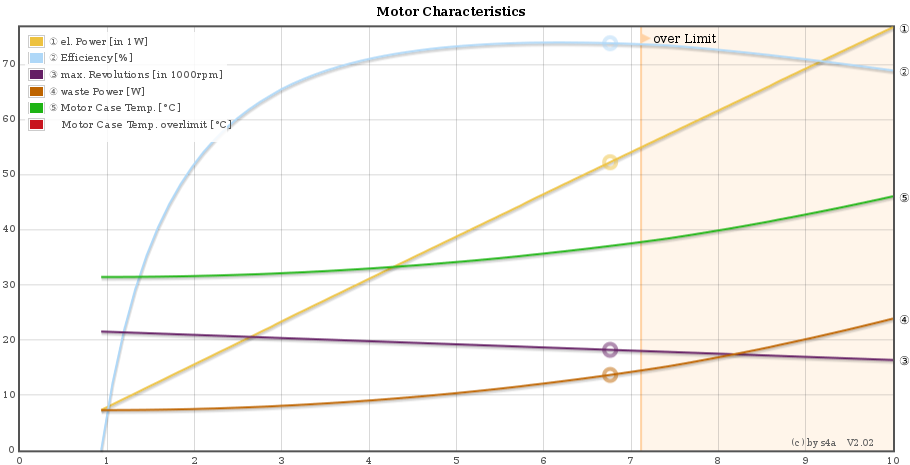
\includegraphics[width=1\textwidth]{../../fig/motor/ecalc_A10-12S.png}
	\caption{Berechnete Kennlinien des Hacker A10-12S}
	\label{fig:ecalc_A10-12S}
\end{figure}


\newpage
\subsubsection*{Hacker A20-12XL EVO}

\begin{table}[h!]
	\centering
	\begin{tabular}{l l l l}
		RC-Parameter & & & \\ \hline
			& Kühlung	& & Mittelmässig \\
			& Batterie	& & LiPo 10Ah, voll, 3S1P, 3.7V \\
			& Regler	& & 30A \\
			& Propeller	& & $\O=10"$, $p=5"$, $b=2$, $p_c=1.3$, $g_r=1$ \\
			& & & \\
		Resultate (max.) & & & \\ \hline
			& Motorstrom	& $I$	& 24.74 A \\
			& Motorspannung	& $U$	& 11.46 V \\
			& Drehzahl	& $n$	& 9676 min$^{-1}$ \\
			& Leistung 	& $P_e$	& 283.5 W \\
			&		& $P_m$	& 225.2 W \\
			& Wikungsgrad	& $\eta$& 79.4 \% \\
			& Motortemperatur
					& $T$	& 52 C \\
			& & & \\
		Berechnungen & & & \\ \hline
			& Winkelgeschwindigkeit
					& $\omega_m$	& 1013.3 s$^{-1}$ \\
			& Drehmoment	& $M$		& 0.222 Nm
	\end{tabular}
	\caption{Simulationsdaten des Hacker A20-12XL-EVO}
\end{table}

\begin{figure}[h!]
	\centering
	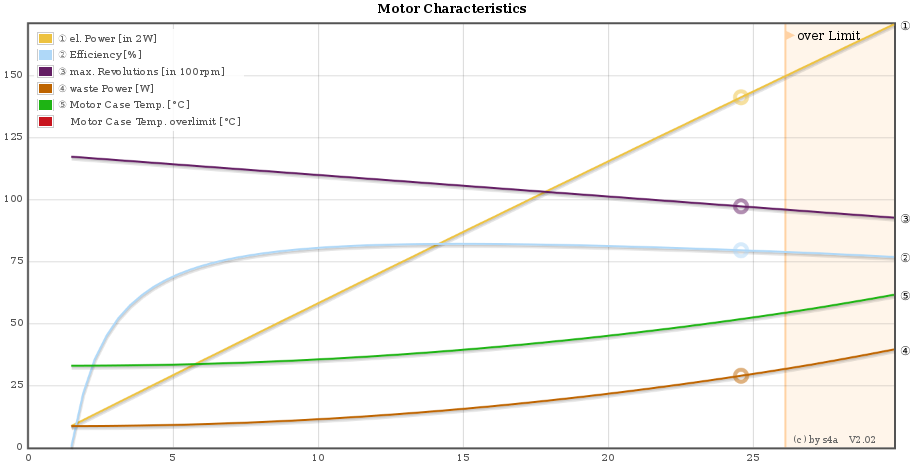
\includegraphics[width=1\textwidth]{../../fig/motor/ecalc_A20-12XL-EVO.png}
	\caption{Berechnete Kennlinien des Hacker A20-12XL-EVO}
	\label{fig:ecalc_A20-12XL-EVO}
\end{figure}


\newpage
\subsubsection*{Hacker A20-20L}

\begin{table}[h!]
	\centering
	\begin{tabular}{l l l l}
		RC-Parameter & & & \\ \hline
			& Kühlung	& & Mittelmässig \\
			& Batterie	& & LiPo 10Ah, voll, 3S1P, 3.7V \\
			& Regler	& & 30A \\
			& Propeller	& & $\o=10"$, $p=5"$, $b=2$, $p_c=1.3$, $g_r=1$ \\
			& & & \\
		Resultate (max.) & & & \\ \hline
			& Motorstrom	& $I$	& 21.2 A \\
			& Motorspannung	& $U$	& 11.5 V \\
			& Drehzahl	& $n$	& 9111 min$^{-1}$ \\
			& Leistung 	& $P_e$	& 243.8 W \\
			&		& $P_m$	& 186.4 W \\
			& Wikungsgrad	& $\eta$& 76.5 \% \\
			& Motortemperatur
					& $T$	& 56 C \\
			& & & \\
		Berechnungen & & & \\ \hline
			& Winkelgeschwindigkeit
					& $\omega_m$	& 954.1 s$^{-1}$ \\
			& Drehmoment	& $M$		& 0.195 Nm
	\end{tabular}
	\caption{Simulationsdaten des Hacker A20-20L}
\end{table}

\begin{figure}[h!]
	\centering
	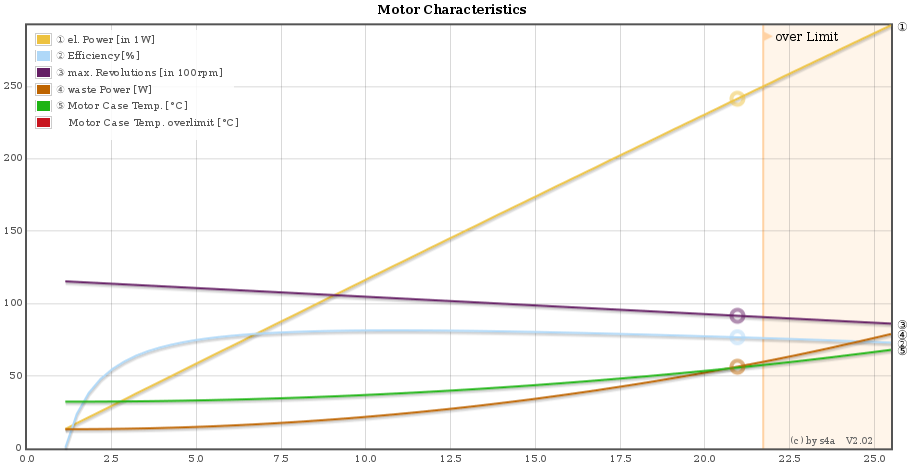
\includegraphics[width=1\textwidth]{../../fig/motor/ecalc_A20-20L.png}
	\caption{Berechnete Kennlinien des Hacker A20-20L}
	\label{fig:ecalc_A20-20L}
\end{figure}


\newpage
\subsubsection*{Dualsky XM3548EA-5}

\begin{table}[h!]
	\centering
	\begin{tabular}{l l l l}
		RC-Parameter & & & \\ \hline
			& Kühlung	& & Mittelmässig \\
			& Batterie	& & LiPo 8Ah, voll, 3S1P, 3.7V \\
			& Regler	& & 40A \\
			& Propeller	& & $\o=13"$, $p=6"$, $b=2$, $p_c=1.3$, $g_r=1$ \\
			& & & \\
		Resultate (max.) & & & \\ \hline
			& Motorstrom	& $I$	& 37.17 A \\
			& Motorspannung	& $U$	& 11.33 V \\
			& Drehzahl	& $n$	& 7467 min$^{-1}$ \\
			& Leistung 	& $P_e$	& 421.1 W \\
			&		& $P_m$	& 359.9 W \\
			& Wikungsgrad	& $\eta$& 85.5 \% \\
			& Motortemperatur
					& $T$	& 50 C \\
			& & & \\
		Berechnungen & & & \\ \hline
			& Winkelgeschwindigkeit
					& $\omega_m$	& 781.9 s$^{-1}$ \\
			& Drehmoment	& $M$		& 0.46 Nm
	\end{tabular}
	\caption{Simulationsdaten des Dualsky XM3548EA-5}
\end{table}

\begin{figure}[h!]
	\centering
	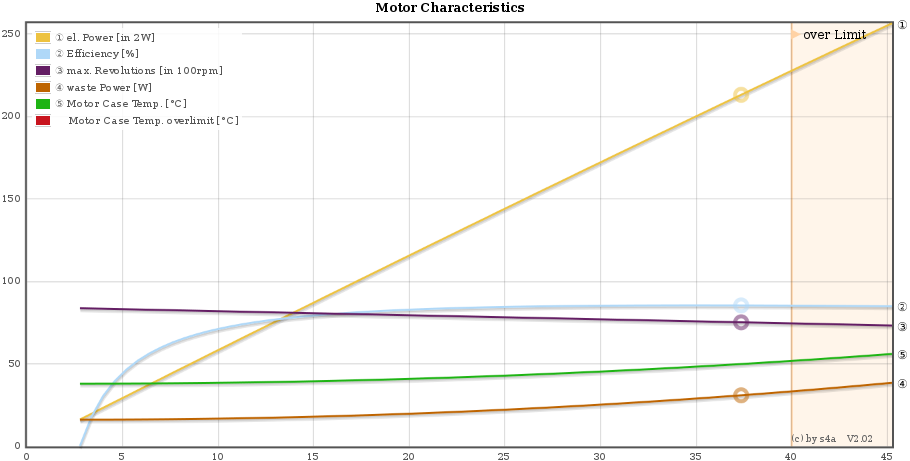
\includegraphics[width=1\textwidth]{../../fig/motor/ecalc_XM3548EA-5.png}
	\caption{Berechnete Kennlinien des Dualsky XM3548EA-5}
	\label{fig:ecalc_xm3548ea_5}
\end{figure}

\newpage

\subsection{Gleichstrommotor}
Der Gleichstrommotor dient dem Ballvorschub, somit muss dieser Motor
eine gewisse Geschwindigkeit haben und eine bestimmte Kraft um die
Wurfobjekte zu bewegen. Um einen passenden Gleichstrommotor zu evaluieren
bedarf es der relevanten mechanischen Daten, wie etwa dem Drehmoment und
der Winkelgeschwindigkeit. Diese Daten sind im Abschnitt
\ref{sec:berechnungen} dargelegt mit den getroffenen Annahmen für die
Berechnungen.

Die Resultate dieser Berechnungen deuten auf einen relativ grossen Motor
hin mit der Annahme, dass dieser ein per Permanentmagnet fremderregter
Gleichstrommotor ist. Gross heisst in diesem Kontext, dass es kein
typischer und kostengünstiger Motor aus dem Modellbau oder Hobbybereich
ist. In einer ersten Phase gilt es die theoretischen Resultate empirisch zu
überprüfen und dann gegebenenfalls einen Paradigmenwechsel bei der
Motortypwahl einzuleiten. Hierfür steht ein funktionsfähiges
Referenzmodell bereit welches in der Abbildung \ref{fig:refmodel}
dargestellt ist. Dieses kann für die Kraft- und Geschwindigkeitsmessung
verwendet werden kann. Dieses besitzt auch einen Drehzahlgeber auf basis
magnetischer Schalter (Hall-Effekt-Schalter) wie diese auch von PREN-ET Team
vorgesehen sind \cite{pren-et-doc}.

\begin{figure}[h!]
	\centering
	\begin{subfigure}[t]{0.45\textwidth}
		\centering
		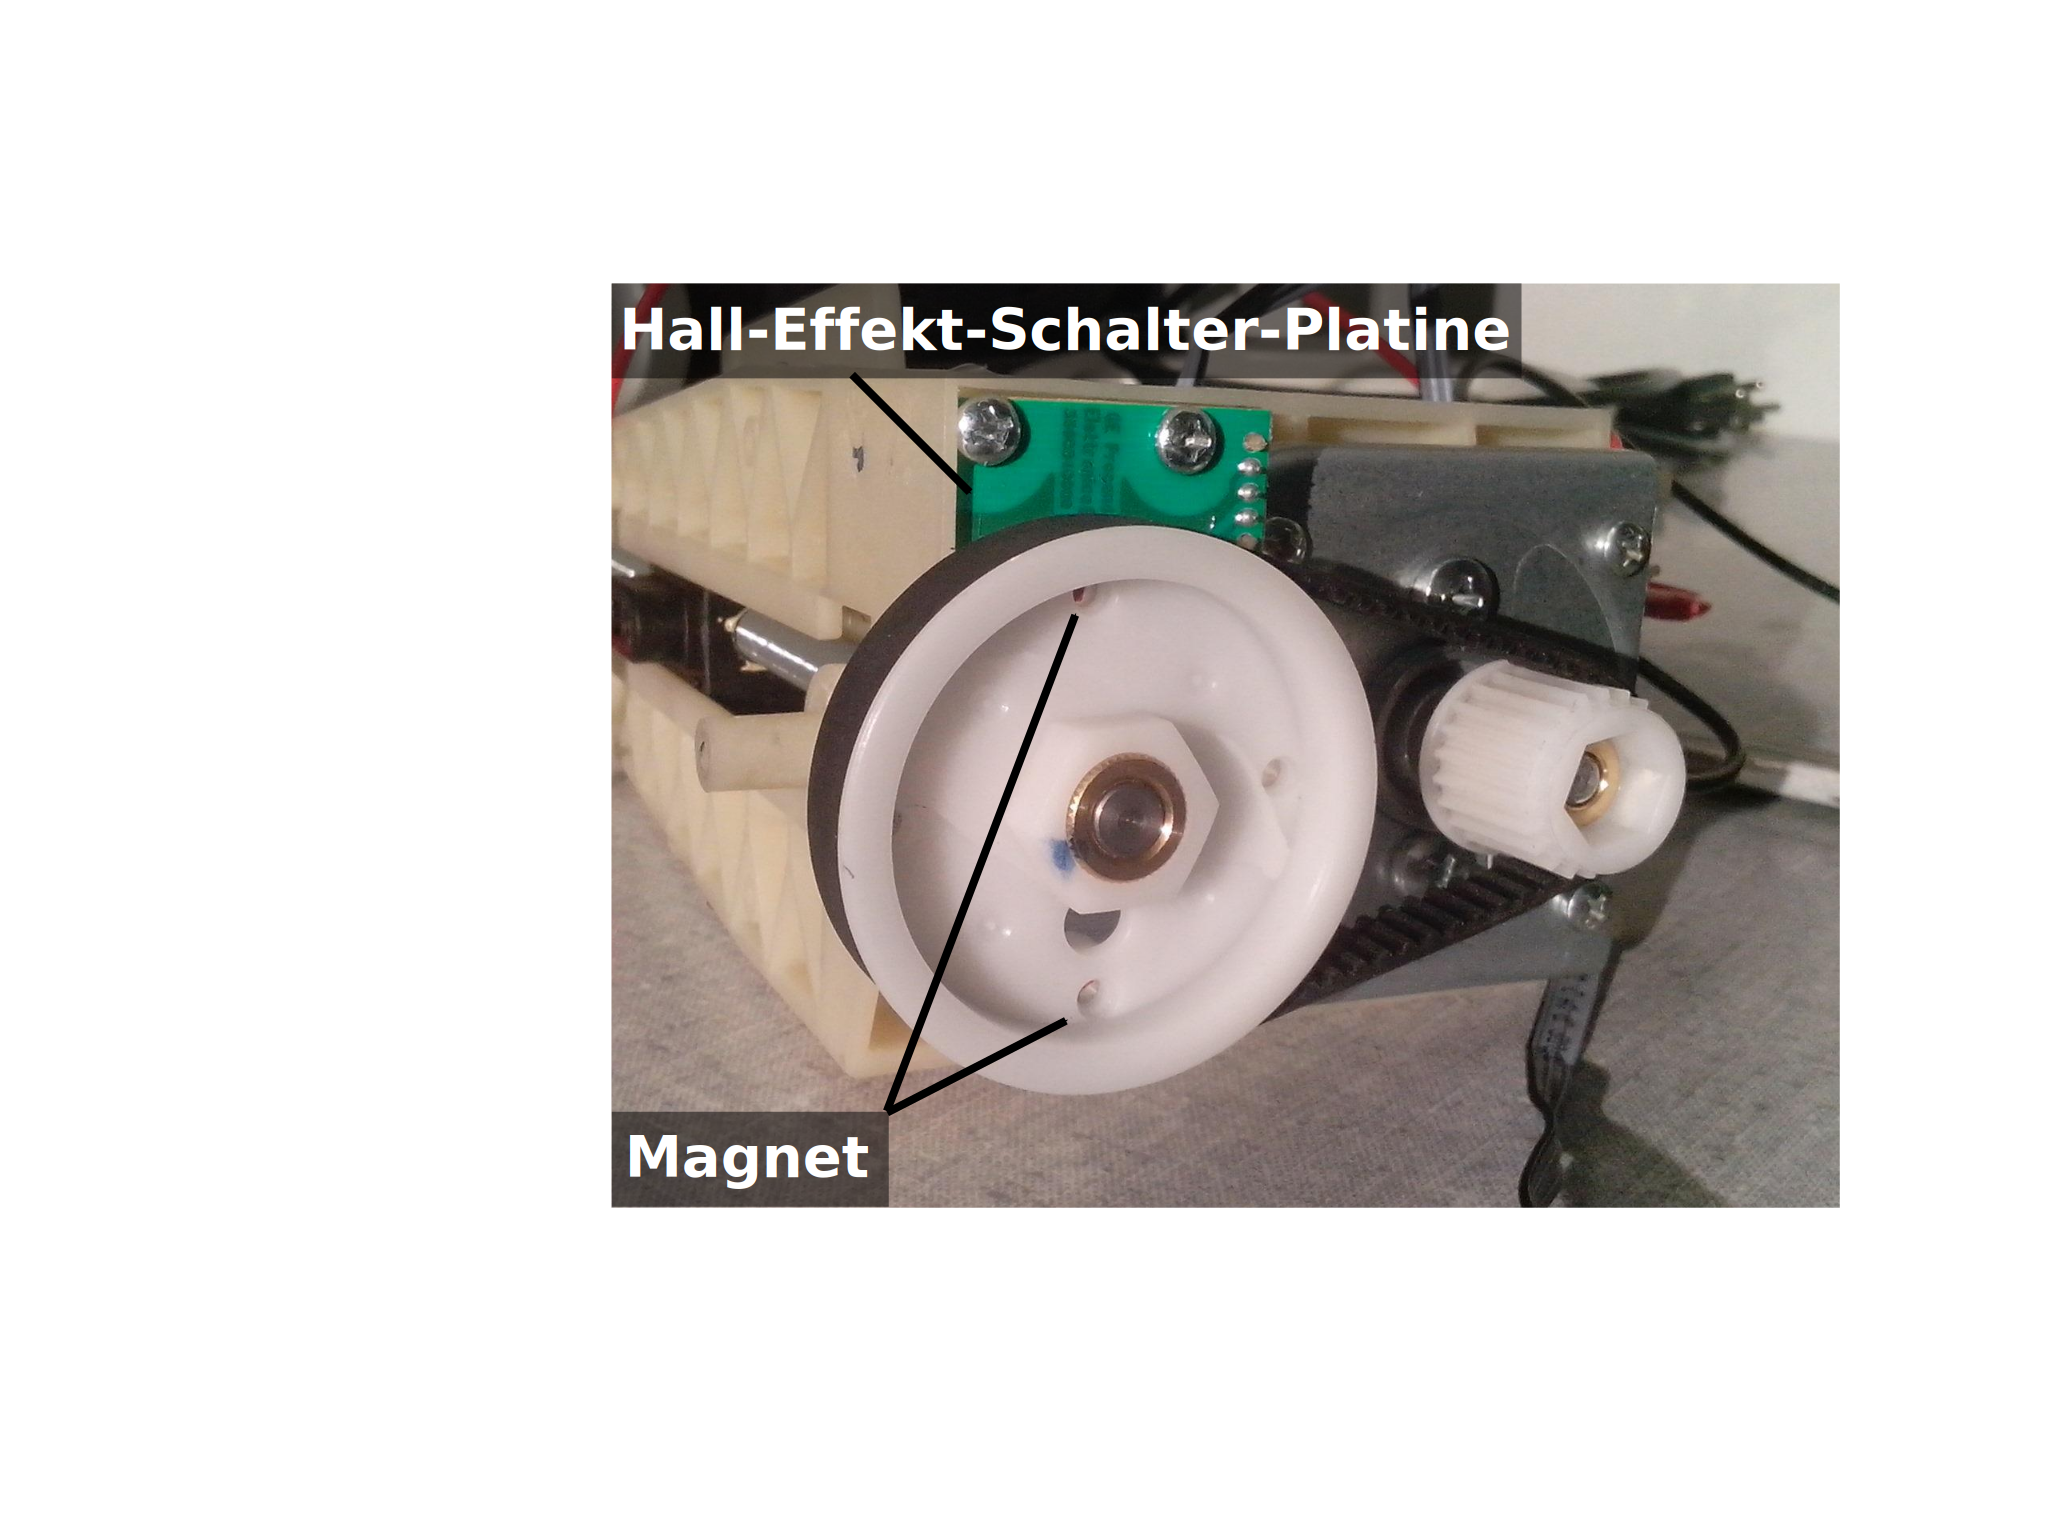
\includegraphics[width=0.95\textwidth]{../../fig/motor/mech-model-03_01.pdf}
		\caption{Untersetzungsgetriebe}
	\end{subfigure}
	\begin{subfigure}[t]{0.45\textwidth}
		\centering
		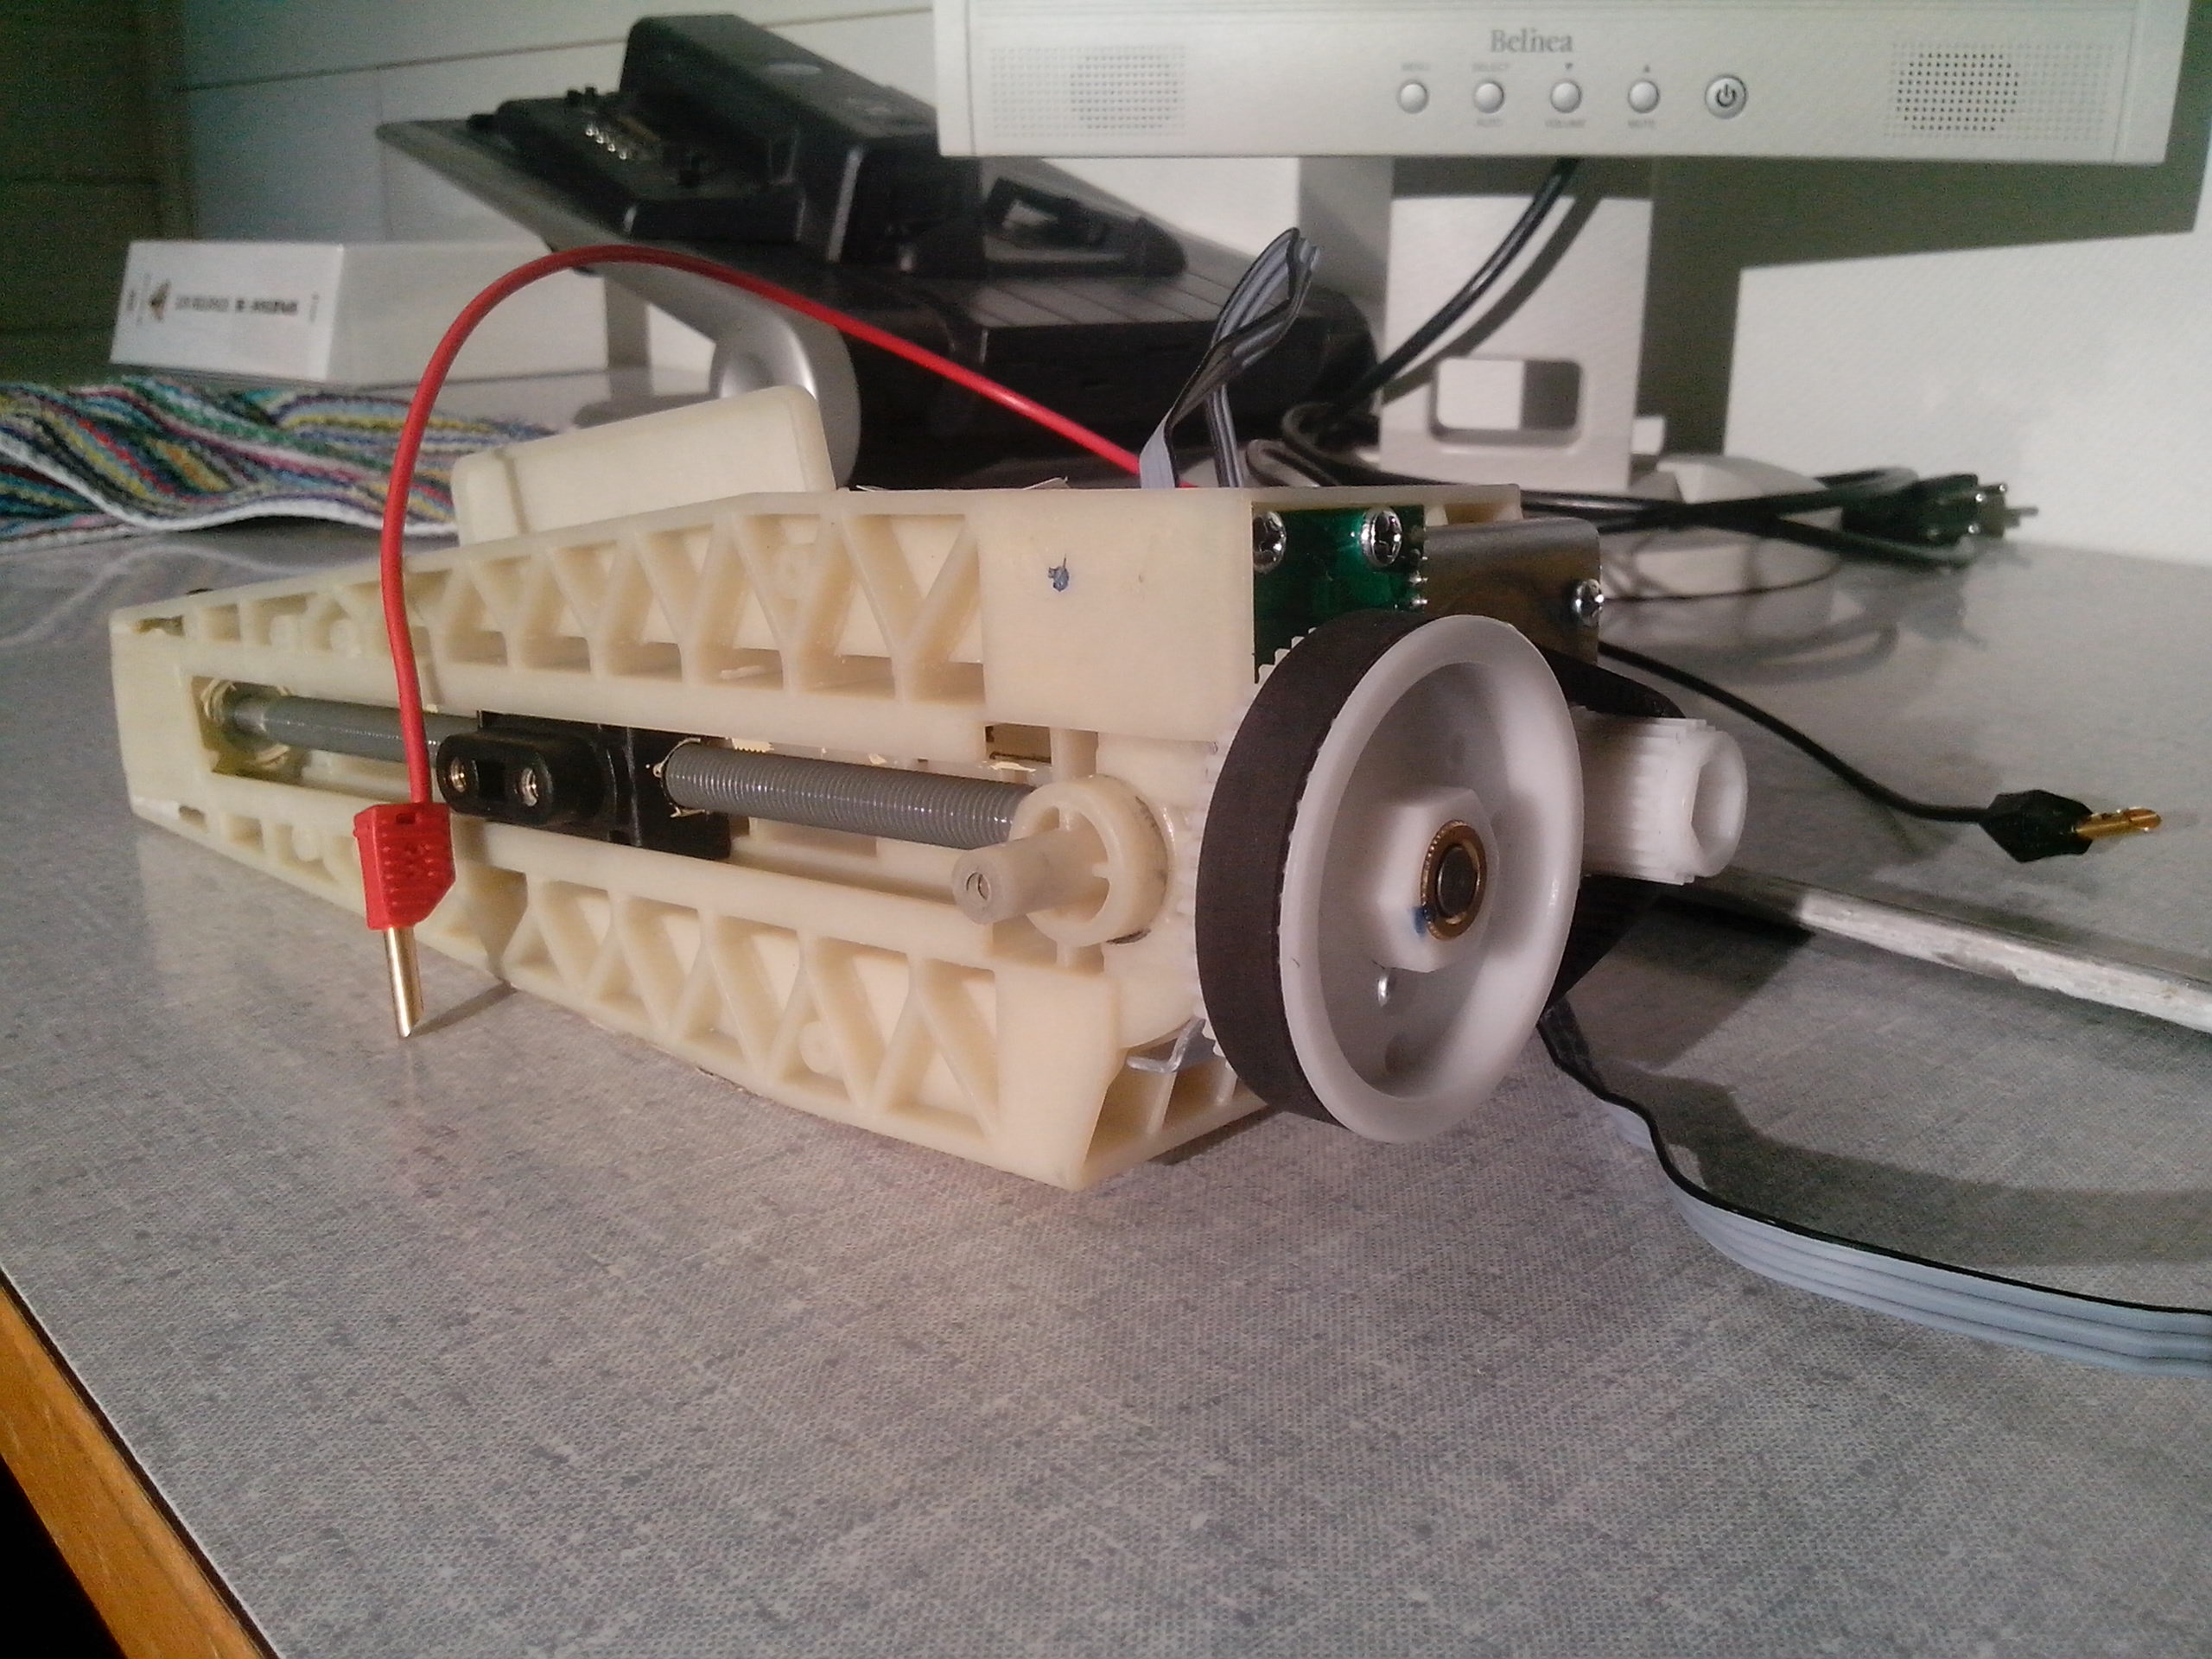
\includegraphics[width=0.95\textwidth]{../../fig/motor/mech-model-02.jpg}
		\caption{Gewindestange mit Gleiter}
	\end{subfigure}

	\begin{comment}
	\begin{subfigure}[t]{0.45\textwidth}
		\centering
		\includegraphics[width=0.95\textwidth]{../../fig/motor/mech-model-}
	\end{subfigure}
	\begin{subfigure}[t]{0.45\textwidth}
		\centering
		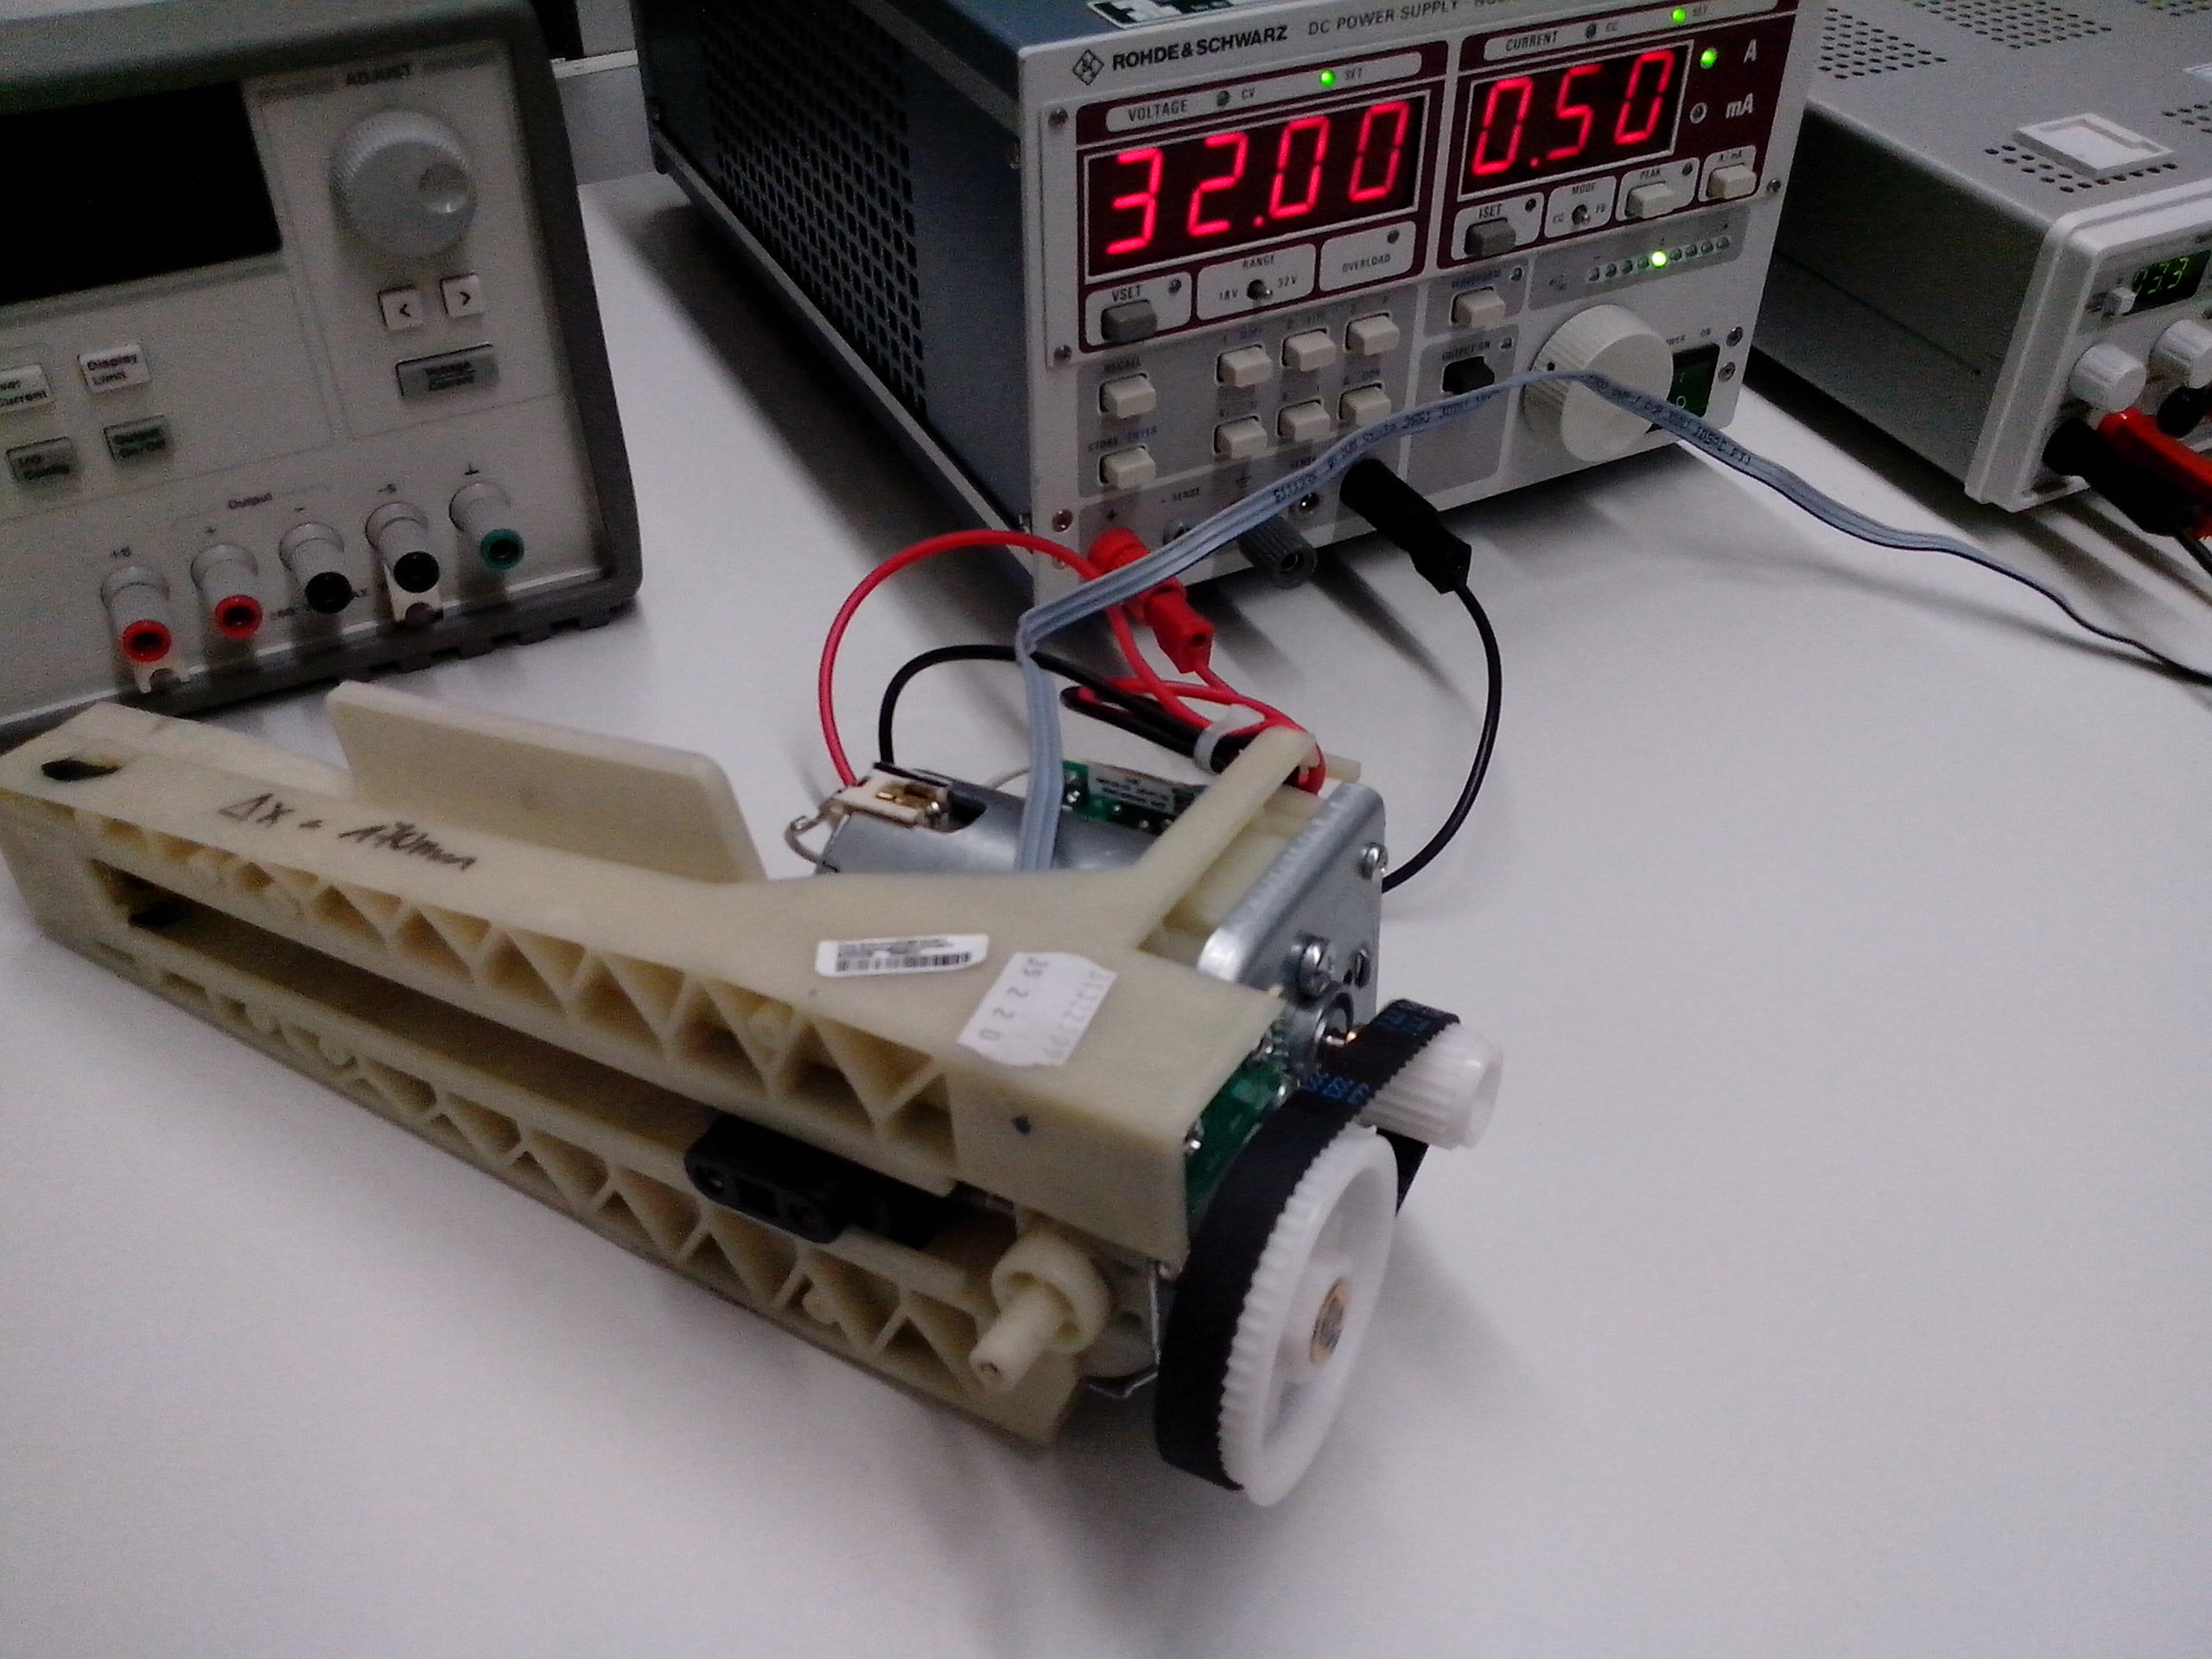
\includegraphics[width=0.95\textwidth]{../../fig/motor/mech-model-05.jpg}
		\caption{Funktionstest mit Labornetzteilen}
	\end{subfigure}
	\end{comment}
	\caption{Funktionsfähiges Referenzmodell für den Ballvorschub}
	\label{fig:refmodel}
\end{figure}

\subsection{Motorentreiber}
Die für die Ansteuerung der Motoren notwendigen Treiber werden innerhalb
einer Fachgruppe von Elektrotechnikern entwickelt. Hierbei gibt es
verschiedene Teams, welche sich jeweils einem der Motorentypen widmen.

Die Organisation dieser Fachgruppe ist offen dargelegt und einsehbar
dokumentiert \cite{pren-et}. Die Dokumentationen sind in einem eigenen
Repository angelegt und öffentlich einsehbar \cite{pren-et-doc}.
